\documentclass[12pt]{article}
\usepackage[a4paper, left=2cm, right=2cm, top=2cm, bottom=2cm]{geometry}
\usepackage{fontspec}
\usepackage{booktabs}
\usepackage{amsmath, amsfonts}
\usepackage{graphicx}
\usepackage{polyglossia}
\usepackage{float}
\setdefaultlanguage{greek}
\setotherlanguage{english}
\setmainfont{Palatino Linotype}
\newfontfamily\greekfonttt{Liberation Mono}[Scale=MatchLowercase]
%\setmonofont{Latin Modern Mono}[Scale=MatchLowercase]
\usepackage{subcaption}
\usepackage{siunitx}
\usepackage{bm}

% This is for code
\usepackage{listings}
\usepackage{xcolor} % Required for custom colors

% This is for CSV
\usepackage{csvsimple-l3}


% Define custom colors
\definecolor{codegreen}{rgb}{0,0.6,0}
\definecolor{codegray}{rgb}{0.5,0.5,0.5}
\definecolor{codepurple}{rgb}{0.58,0,0.82}
\definecolor{backcolour}{rgb}{0.95,0.95,0.92}

% Define a custom style for C code
\lstdefinestyle{CStyle}{
    language=C,
    backgroundcolor=\color{backcolour},   
    commentstyle=\color{codegreen},
    keywordstyle=\color{blue}\bfseries,
    numberstyle=\tiny\color{codegray},
    stringstyle=\color{codepurple},
    basicstyle=\ttfamily\footnotesize,
    breakatwhitespace=false,         
    breaklines=true,                 
    captionpos=b,                    
    keepspaces=true,                 
    numbers=left,                    
    numbersep=5pt,                  
    showspaces=false,                
    showstringspaces=false,
    showtabs=false,                  
    tabsize=4
}

\begin{document}

% --- HEADER START ---
\noindent
\begin{minipage}[t]{\textwidth}
    {\large \textbf{Εθνικό Μετσόβιο Πολυτεχνείο}} \\
    \textbf{Σχολή Ηλεκτρολόγων Μηχανικών και Μηχανικών Υπολογιστών} \\    
    \textbf{Τομέας Τεχνολογίας Πληροφορικής και Υπολογιστών} \\
    Μάθημα: "Σχεδιασμός Ενσωματωμένων Συστημάτων" \\
    Ακαδ. Έτος: 2026-2027
\end{minipage}

\vspace{0.2cm}
\hrule height 1pt
\vspace{1cm}
% --- HEADER END ---


% --- TITLE SECTION ---
\begin{center}
    {\LARGE \textbf{2η Εργαστηριακή Άσκηση}} \\[0.5cm]
    {\large Βελτιστοποίηση Δυναμικών Δομών Δεδομένων (Dynamic Data Type Refinement – DDTR) και Dynamic Memory Management (DMM)}
\end{center}
\vspace{1cm}


% --- AUTHORS SECTION ---
\begin{center}
	\textbf{Αποστολόπουλος Νικόλαος} \\
	(03122614) \\
	\textbf{Γκριμπογιάννης Χαρίλαος} \\
	(03122002)
\end{center}
\vspace{1cm}

% --- ABSTRACT SECTION ---
\begin{center}
    \textbf{\large Περίληψη}
\end{center}

\noindent
Η παρούσα εργασία υλοποιήθηκε στα πλαίσια του μαθήματος "Σχεδιασμός Ενσωματωμένων Συστημάτων" και σκοπεύει στη βελτιστοποίηση των δυναμικών δομών δεδομένων και της δυναμικής διαχείρισης μνήμης του αλγορίθμου Non-Maximum Suppression (NMS) σε νευρωνικό δίκτυο ανίχνευσης αντικειμένων YOLO μέσω της χρήσης των τεχνικών Dynamic Data Type Refinement (DDTR) και Dynamic Memory Management (DMM).
\pagebreak

\tableofcontents
\pagebreak

\section*{Εισαγωγή}
Στα σύγχρονα συστήματα διαχείρισης κυκλοφορίας δύνανται να υπάρχουν "έξυπνες" κάμερες οι οποίες προσαρμόζουν δυναμικά τη λειτουργία των φωτεινών σηματοδοτών. Ένα τέτοιο σύστημα αποτελείται από μία ή περισσότερες κάμερες εγκατεστημένες σε μία διασταύρωση και έναν ενσωματωμένο ελεγκτή (embedded controller) ο οποίος λαμβάνει εικόνες από αυτές τις κάμερες και υπολογίζει τον αριθμό των οχημάτων που κινούνται σε κάθε κατεύθυνση, ούτως ώστε να αποφασίζει πότε πρέπει να αλλάζει η κατάσταση των φωτεινών σηματοδοτών.

Σε ένα τέτοιο σύστημα, η ταχύτητα επεξεργασίας των δεδομένων είναι κρίσιμη ώστε να μην μειώνεται η αποδοτικότητα της κυκλοφορίας. Έτσι, χρησιμοποιούμε την ετερογενή πλατφόρμα AUP-ZU3, όπου το νευρωνικό δίκτυο YOLOv5s εκτελείται στο FPGA, ενώ το post-processing (decoding, εφαρμογή NMS και καταμέτρηση οχημάτων ανά κατεύθυνση) εκτελείται στη CPU.

Η εφαρμογή του αλγορίθμου NMS κρίνεται απαραίτητη, καθώς το μοντέλο YOLO δεν παράγει ένα μοναδικό bounding box για κάθε αντικείμενο, αλλά επιστρέφει ένα σύνολο από candidate boxes συνοδευόμενα το καθένα από την προβλεπόμενη κλάση του αντικειμένου (π.χ. αυτοκίνητο, άνθρωπος) και μια τιμή confidence (βαθμός βεβαιότητας πρόβλεψης). Ο αλγόριθμος NMS είναι υπεύθυνος για την απομάκρυνση των διπλών ανιχνεύσεων.

Στο πλαίσιο της εργαστηριακής αυτής άσκησης, καθώς επικεντρωνόμαστε στη βελτιστοποίηση του αλγορίθμου NMS, χρησιμοποιούμε προ-υπολογισμένα δεδομένα εξόδου του δικτύου YOLOv5s χωρίς να το εκτελούμε. Οι επιμέρους στόχοι της άσκησης είναι η βελτιστοποίηση του συνολικού χρόνου εκτέλεσης της εφαρμογής NMS (execution time), η βελτιστοποίηση των συνολικών προσβάσεων (reads/writes) της κύριας μνήμης (memory accesses) και η βελτιστοποίηση της μέγιστης ποσότητας κύριας μνήμης που καταλαμβάνει η εφαρμογή (memory footprint).

\section{Εκτέλεση της Αρχικής Έκδοσης της Εφαρμογής NMS}
Για να έχουμε ένα baseline με το οποίο θα συγκρίνουμε την απόδοση της δικής μας υλοποίησης, εκτελούμε την αρχική έκδοση της εφαρμογής NMS, η οποία χρησιμοποιεί το container \texttt{std::vector<Detection>} για την αποθήκευση των candidate boxes κάθε κλάσης  και τη default έκδοση της \texttt{glibc} ως allocator για τη δυναμική διαχείριση μνήμης.

Ξεκινάμε με confidence threshold $0.05$ και εκτελώντας την αρχική έκδοση της εφαρμογής $20$ φορές βρίσκουμε ότι ο μέσος χρόνος εκτέλεσης είναι \qty{347.30}{\milli\second} με variance \qty{0.348}{\milli\second\squared}, το οποίο επιβεβαιώνει ότι οι μετρήσεις μας είναι σταθερές και επαναλήψιμες.

Τέλος, μετράμε τη συνολική μνήμη που χρησιμοποιεί το NMS (σε ξεχωριστή εκτέλεση) και βρίσκουμε ότι το heap size που χρησιμοποιεί το NMS είναι \qty{295936}{B}.

\section{Βελτιστοποίηση Δυναμικών Δομών Δεδομένων του Αλγορίθμου NMS}
Στην παρούσα παράγραφο μελετάμε την επίδραση 9 διαφορετικών δομών δεδομένων της βιβλιοθήκης DDTR στον χρόνο εκτέλεσης και το memory footprint της εφαρμογής NMS. Μελετάμε τις εξής δομές:
\begin{itemize}
\item Vector
\item Single Linked List (SLL) (\texttt{single\_linked\_list})
\item Double Linked List (DLL) (\texttt{double\_linked\_list})
\item SLL με roving pointer (SLLR) (\texttt{roving\_single\_linked\_list})
\item DLL με roving pointer (DLLR) (\texttt{roving\_double\_linked\_list})
\item SLL χωρίς sentinel κόμβο (\texttt{single\_linked\_list\_no\_sentinel})
\item DLL χωρίς sentinel κόμβο (\texttt{double\_linked\_list\_no\_sentinel})
\item SLLR χωρίς sentinel κόμβο (\texttt{roving\_single\_linked\_list\_no\_sentinel})
\item DLLR χωρίς sentinel κόμβο (\texttt{roving\_double\_linked\_list\_no\_sentinel})
\end{itemize}

Αφού τροποποιήσουμε τον κώδικα, μεταγλωττίσουμε και ελέγξουμε την ορθότητα της λύσης μας, εκτελούμε την εφαρμογή με όλους τους διαφορετικούς συνδυασμούς υλοποιήσεων δομών δεδομένων για το NMS και καταγράφουμε τα αποτελέσματα κάθε συνδυασμού σχετικά με το μέγεθος της απαιτούμενης μνήμης (memory footprint), τον χρόνο εκτέλεσης και τα LLC misses του perf.

\begin{table}[H]
    \centering
    \resizebox{\textwidth}{!}{%
    \csvreader[
        tabular=lcccccc,
        table head=\toprule Δομή Δεδομένων (DDT) & Χρόνος (ms) & Var ($\text{ms}^2$) & Memory (B) & LLC (full) & LLC (\texttt{runs=0}) & Net LLC ($\Delta$) \\\midrule,
        table foot=\bottomrule,
        late after line=\\
    ]{ddtr_q2_results.csv}{}
    {\csvcoli & \csvcolii & \csvcoliii & \csvcoliv & \csvcolv & \csvcolvi & \csvcolvii}%
    }
    \caption{Μετρήσεις Απόδοσης, Μνήμης και LLC Misses για τις 9 Δομές Δεδομένων και την Αρχική Υλοποίηση ($3\times20 = 60$ runs)}
    \label{tab:q2-ddts}
\end{table}

Από τις μετρήσεις του Πίνακα \ref{tab:q2-ddts} παρατηρούμε ότι η έκδοση της εφαρμογής που ελαχιστοποιεί τον χρόνο εκτέλεσης είναι αυτή που χρησιμοποιεί DLLR χωρίς sentinel κόμβο με χρόνο εκτέλεσης \qty{86.50}{\milli\second}, ενώ η έκδοση που ελαχιστοποιεί το συνολικό memory footprint είναι αυτή με SLL χωρίς sentinel κόμβο (\qty{148224}{B}).

Στο Σχήμα \ref{fig:q2-pareto} παρατηρούμε ότι το Pareto Frontier αποτελείται από τις τέσσερις υλοποιήσεις λιστών χωρίς sentinel κόμβο: την SLL χωρίς sentinel (\qty{148224}{B}, \qty{103.94}{\milli\second}), την SLLR χωρίς sentinel (\qty{148320}{B}, \qty{102.80}{\milli\second}), την DLL χωρίς sentinel (\qty{155616}{B}, \qty{87.12}{\milli\second}) και την DLLR χωρίς sentinel (\qty{155712}{B}, \qty{86.50}{\milli\second}). Σε σύγκριση με την αρχική υλοποίηση (\qty{347.39}{\milli\second}, \qty{295936}{B}), η ταχύτερη λύση (DLLR χωρίς sentinel) επιτυγχάνει speedup $4.02\times$ (μείωση χρόνου κατά $75.10\%$) και μείωση μνήμης κατά $47.38\%$, ενώ η SLL χωρίς sentinel μειώνει τη μνήμη κατά $49.91\%$ με speedup $3.34\times$.

Η υπεροχή των συνδεδεμένων λιστών έναντι του \texttt{std::vector} και του Vector οφείλεται σε δύο παράγοντες: Πρώτον, κατά το \texttt{erase()} στον εμφωλευμένο βρόχο του NMS, το vector αναγκάζεται να μετακινεί σειριακά στη μνήμη όλα τα επόμενα στοιχεία μεγέθους \qty{152}{B} ($O(N)$), ενώ οι λίστες ενημερώνουν απλώς δείκτες. Δεύτερον, οι δυναμικοί διπλασιασμοί χωρητικότητας του vector δεσμεύουν σχεδόν διπλάσια μνήμη από όση απαιτείται, ενώ οι λίστες δεσμεύουν ακριβώς έναν κόμβο ανά candidate box. Μεταξύ των λιστών, οι διπλά συνδεδεμένες (DLL/DLLR) είναι ταχύτερες κατά $\sim$\qty{16}{\milli\second} από τις SLL/SLLR χάρη στη διαγραφή σε χρόνο $O(1)$ μέσω του δείκτη \texttt{prev}, με μικρό επιπλέον κόστος μνήμης ($\sim$\qty{7.4}{kB}). Επιπλέον, η απουσία sentinel κόμβων εξοικονομεί μνήμη και χρόνο σε όλες τις λίστες, ενώ οι καθαρές αστοχίες της LLC ($\Delta$) παραμένουν σχεδόν ίδιες ($184{,}811$ με $187{,}348$) καθώς το ενεργό working set χωράει στην L2 cache.

\begin{figure} [H]
\centering
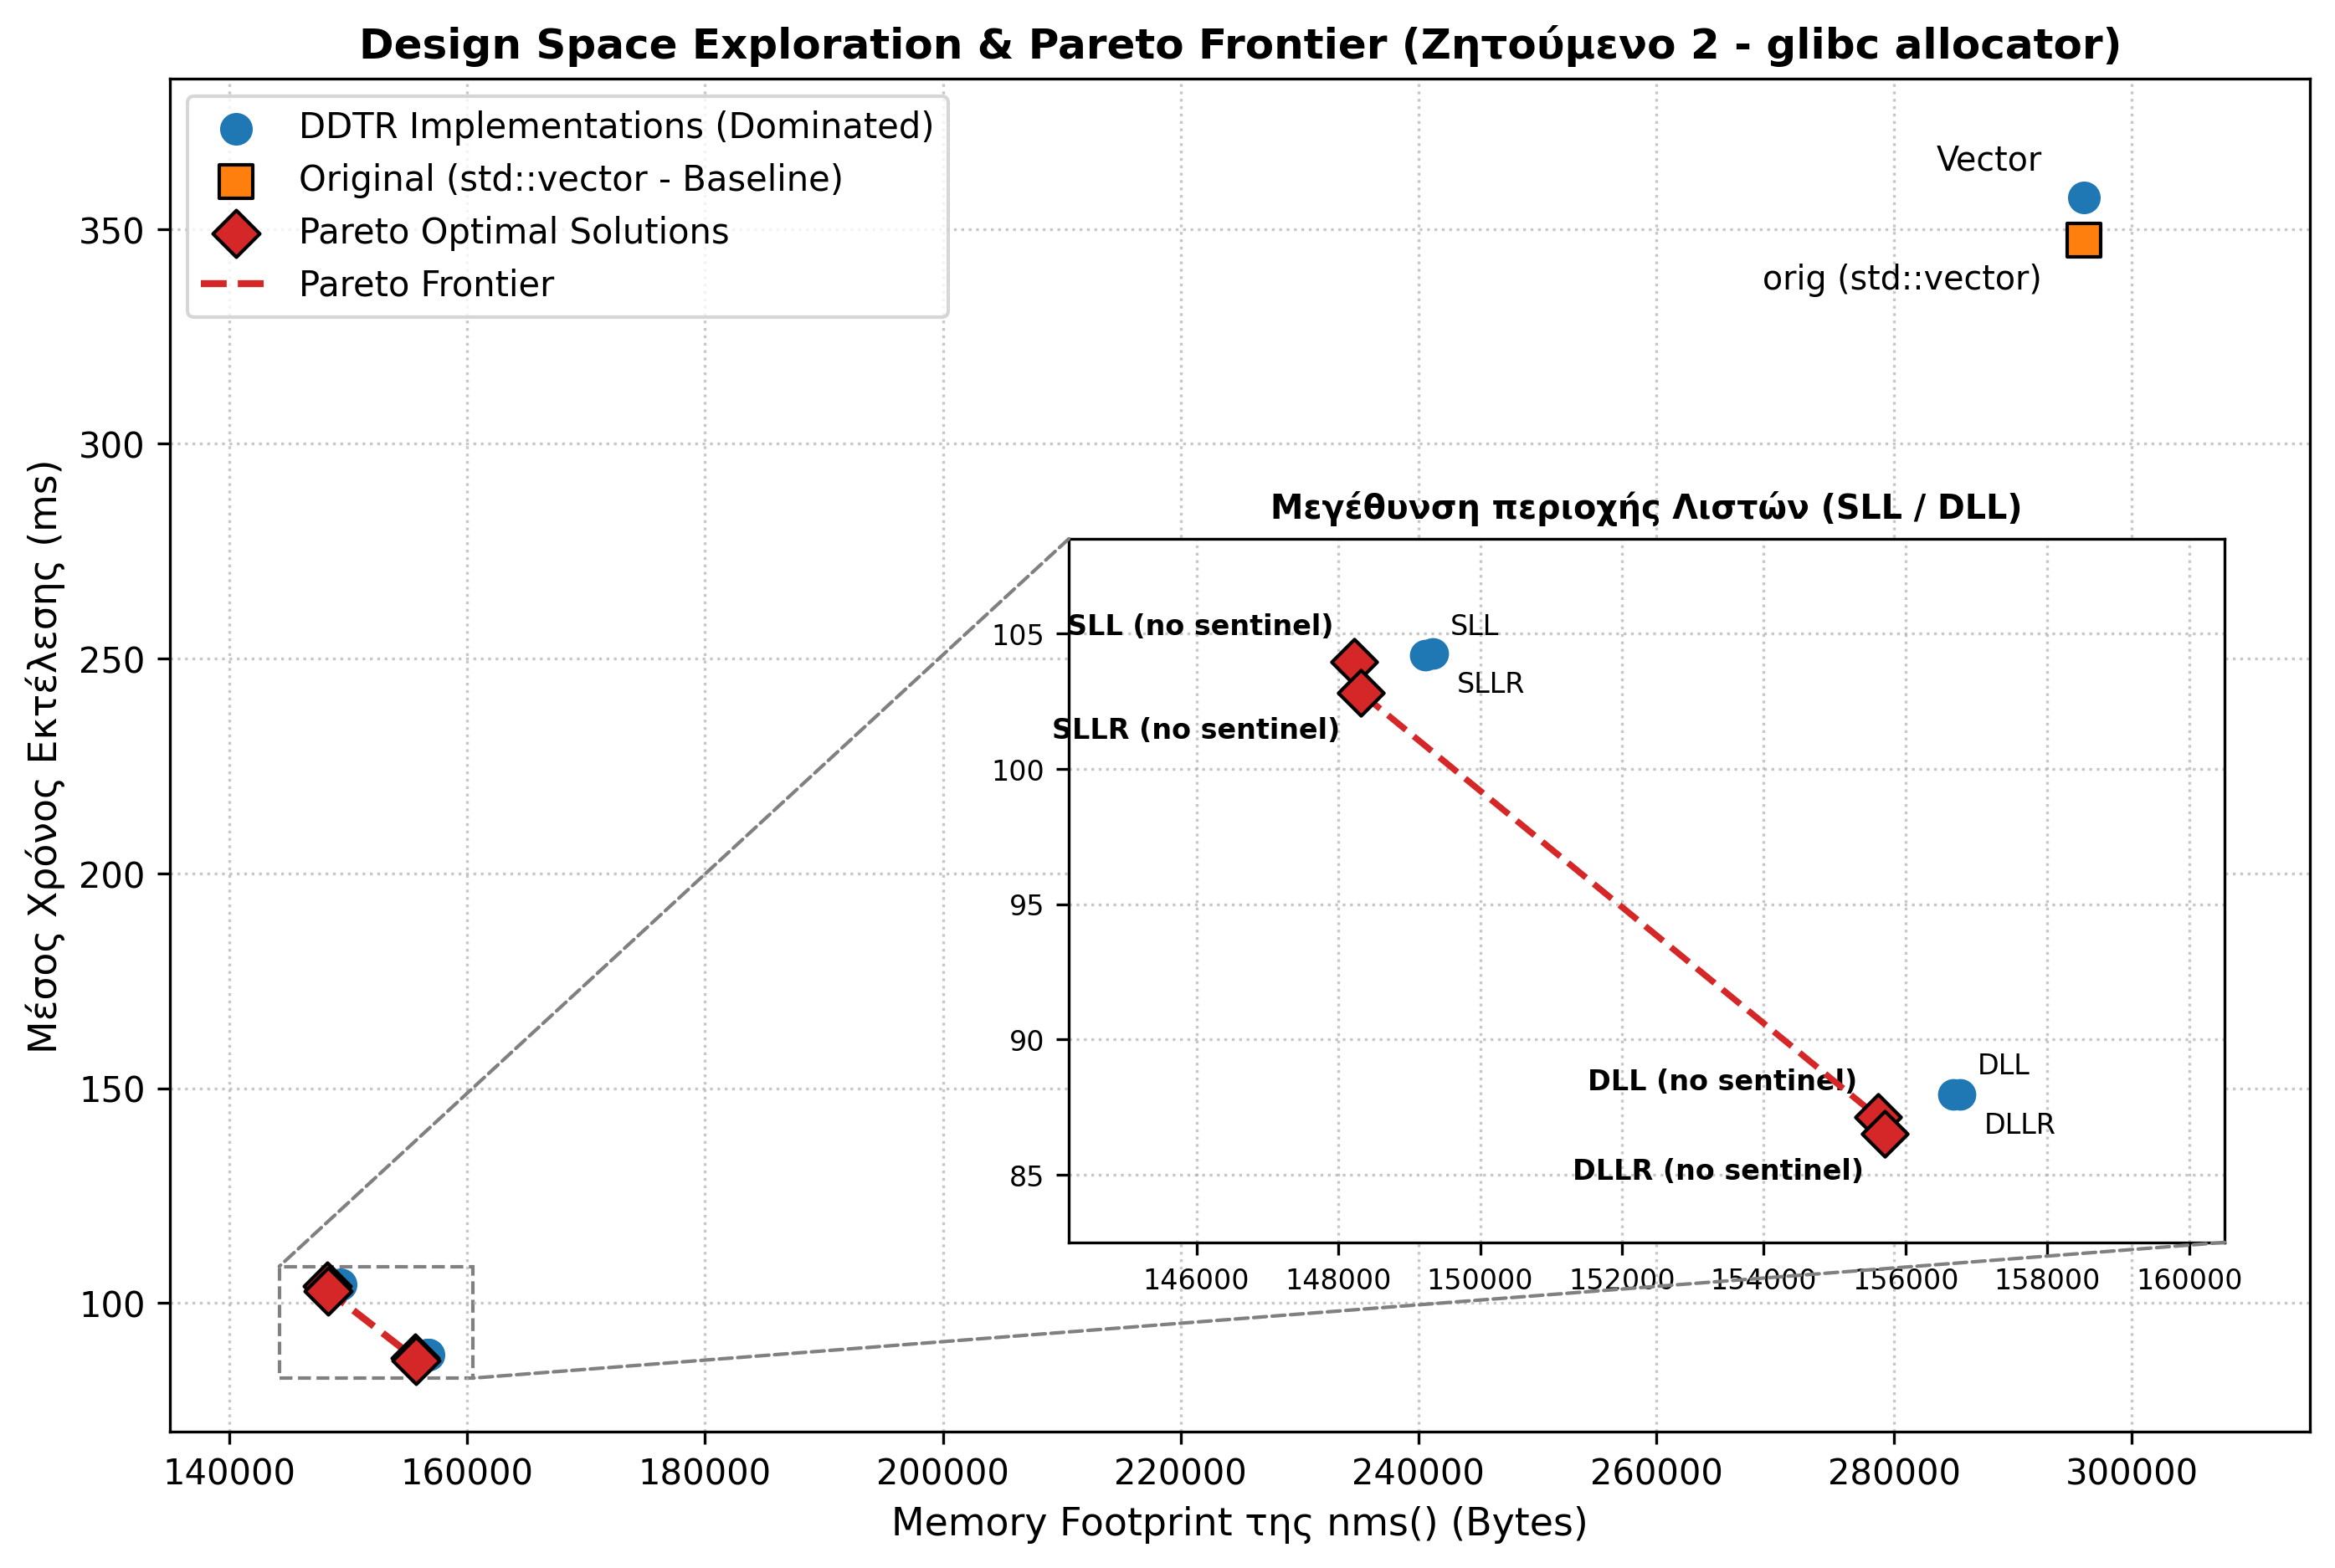
\includegraphics[width=0.8\linewidth]{pareto_q2}
\caption{Pareto Frontier (Ζητούμενο 2 - glibc allocator)}
\label{fig:q2-pareto}
\end{figure}


%\lstinputlisting[style=CStyle, caption={Source Code (tables.c)}, label={lst:tables}]{tables.c}


%\begin{lstlisting}[style=CStyle, caption=Loop Unrolling with Unrolling Factor k, label=lst:loop-unrolling]
%for (i = 0; i <= N - k; i = i + k) {
%	y[i] = y[i] + a1 * x1[i] + a2 * x2[i] + a3 * x3[i];
%	...	
%    y[(i + k)] = y[(i + k)] + a1 * x1[(i + k)] + a2 * x2[(i + k)] + a3 * x3[(i + k)];
%}
%for (int i = N - ((N - (0)) % k); i <= N - 1; i = %i + 1) 
%	y[i] = y[i] + a1 * x1[i] + a2 * x2[i] + a3 * %x3[i];
%\end{lstlisting}

\section{Χρήση Διαφορετικών Allocators}
Μέχρι στιγμής, για τη δυναμική διαχείριση μνήμης χρησιμοποιείται η default έκδοση της \texttt{glibc} ως allocator. Στην παρούσα παράγραφο εξετάζουμε την επίδραση διαφορετικών allocators στον χρόνο εκτέλεσης και τη χρήση της μνήμης της εφαρμογής NMS. Οι allocators που εξετάζουμε είναι οι εξής:
\begin{itemize}
\item \texttt{worst\_fit\_allocator}
\item \texttt{arena\_allocator}
\item \texttt{first\_fit\_allocator}
\item \texttt{best\_fit\_allocator}
\end{itemize}

Ο \texttt{worst\_fit\_allocator} είναι ήδη υλοποιημένος, οπότε υλοποιούμε τους άλλους τρεις και για κάθε συνδυασμό DDT (οι 9 της προηγούμενης παραγράφου) και allocation policy εκτελούμε την εφαρμογή και καταγράφουμε τον χρόνο εκτέλεσης, το memory footprint και το πλήθος των προσβάσεων στη μνήμη. Από τις μετρήσεις αυτές (βλ. Πίνακα \ref{tab:q3-results}) δημιουργείται το Pareto plot του Σχήματος \ref{fig:q3-pareto}.

\begin{table}[H]
    \centering
    \scriptsize
    \renewcommand{\arraystretch}{0.88}
    \resizebox{\textwidth}{!}{%
    \csvreader[
        tabular=llccccccc,
        table head=\toprule Allocator & DDT & Χρόνος (ms) & Var ($\text{ms}^2$) & Mem (B) & mmap (B) & LLC & LLC (\texttt{runs=0}) & Net LLC ($\Delta$) \\\midrule,
        table foot=\bottomrule,
        late after line=\\
    ]{ddtr_q3_results.csv}{}
    {\csvcoli & \csvcolii & \csvcoliii & \csvcoliv & \csvcolv & \csvcolvi & \csvcolvii & \csvcolviii & \csvcolix}%
    }
    \caption{Μετρήσεις απόδοσης, μνήμης και προσβάσεων κύριας μνήμης για το Ζητούμενο 3}
    \label{tab:q3-results}
\end{table}

\begin{figure} [H]
\centering
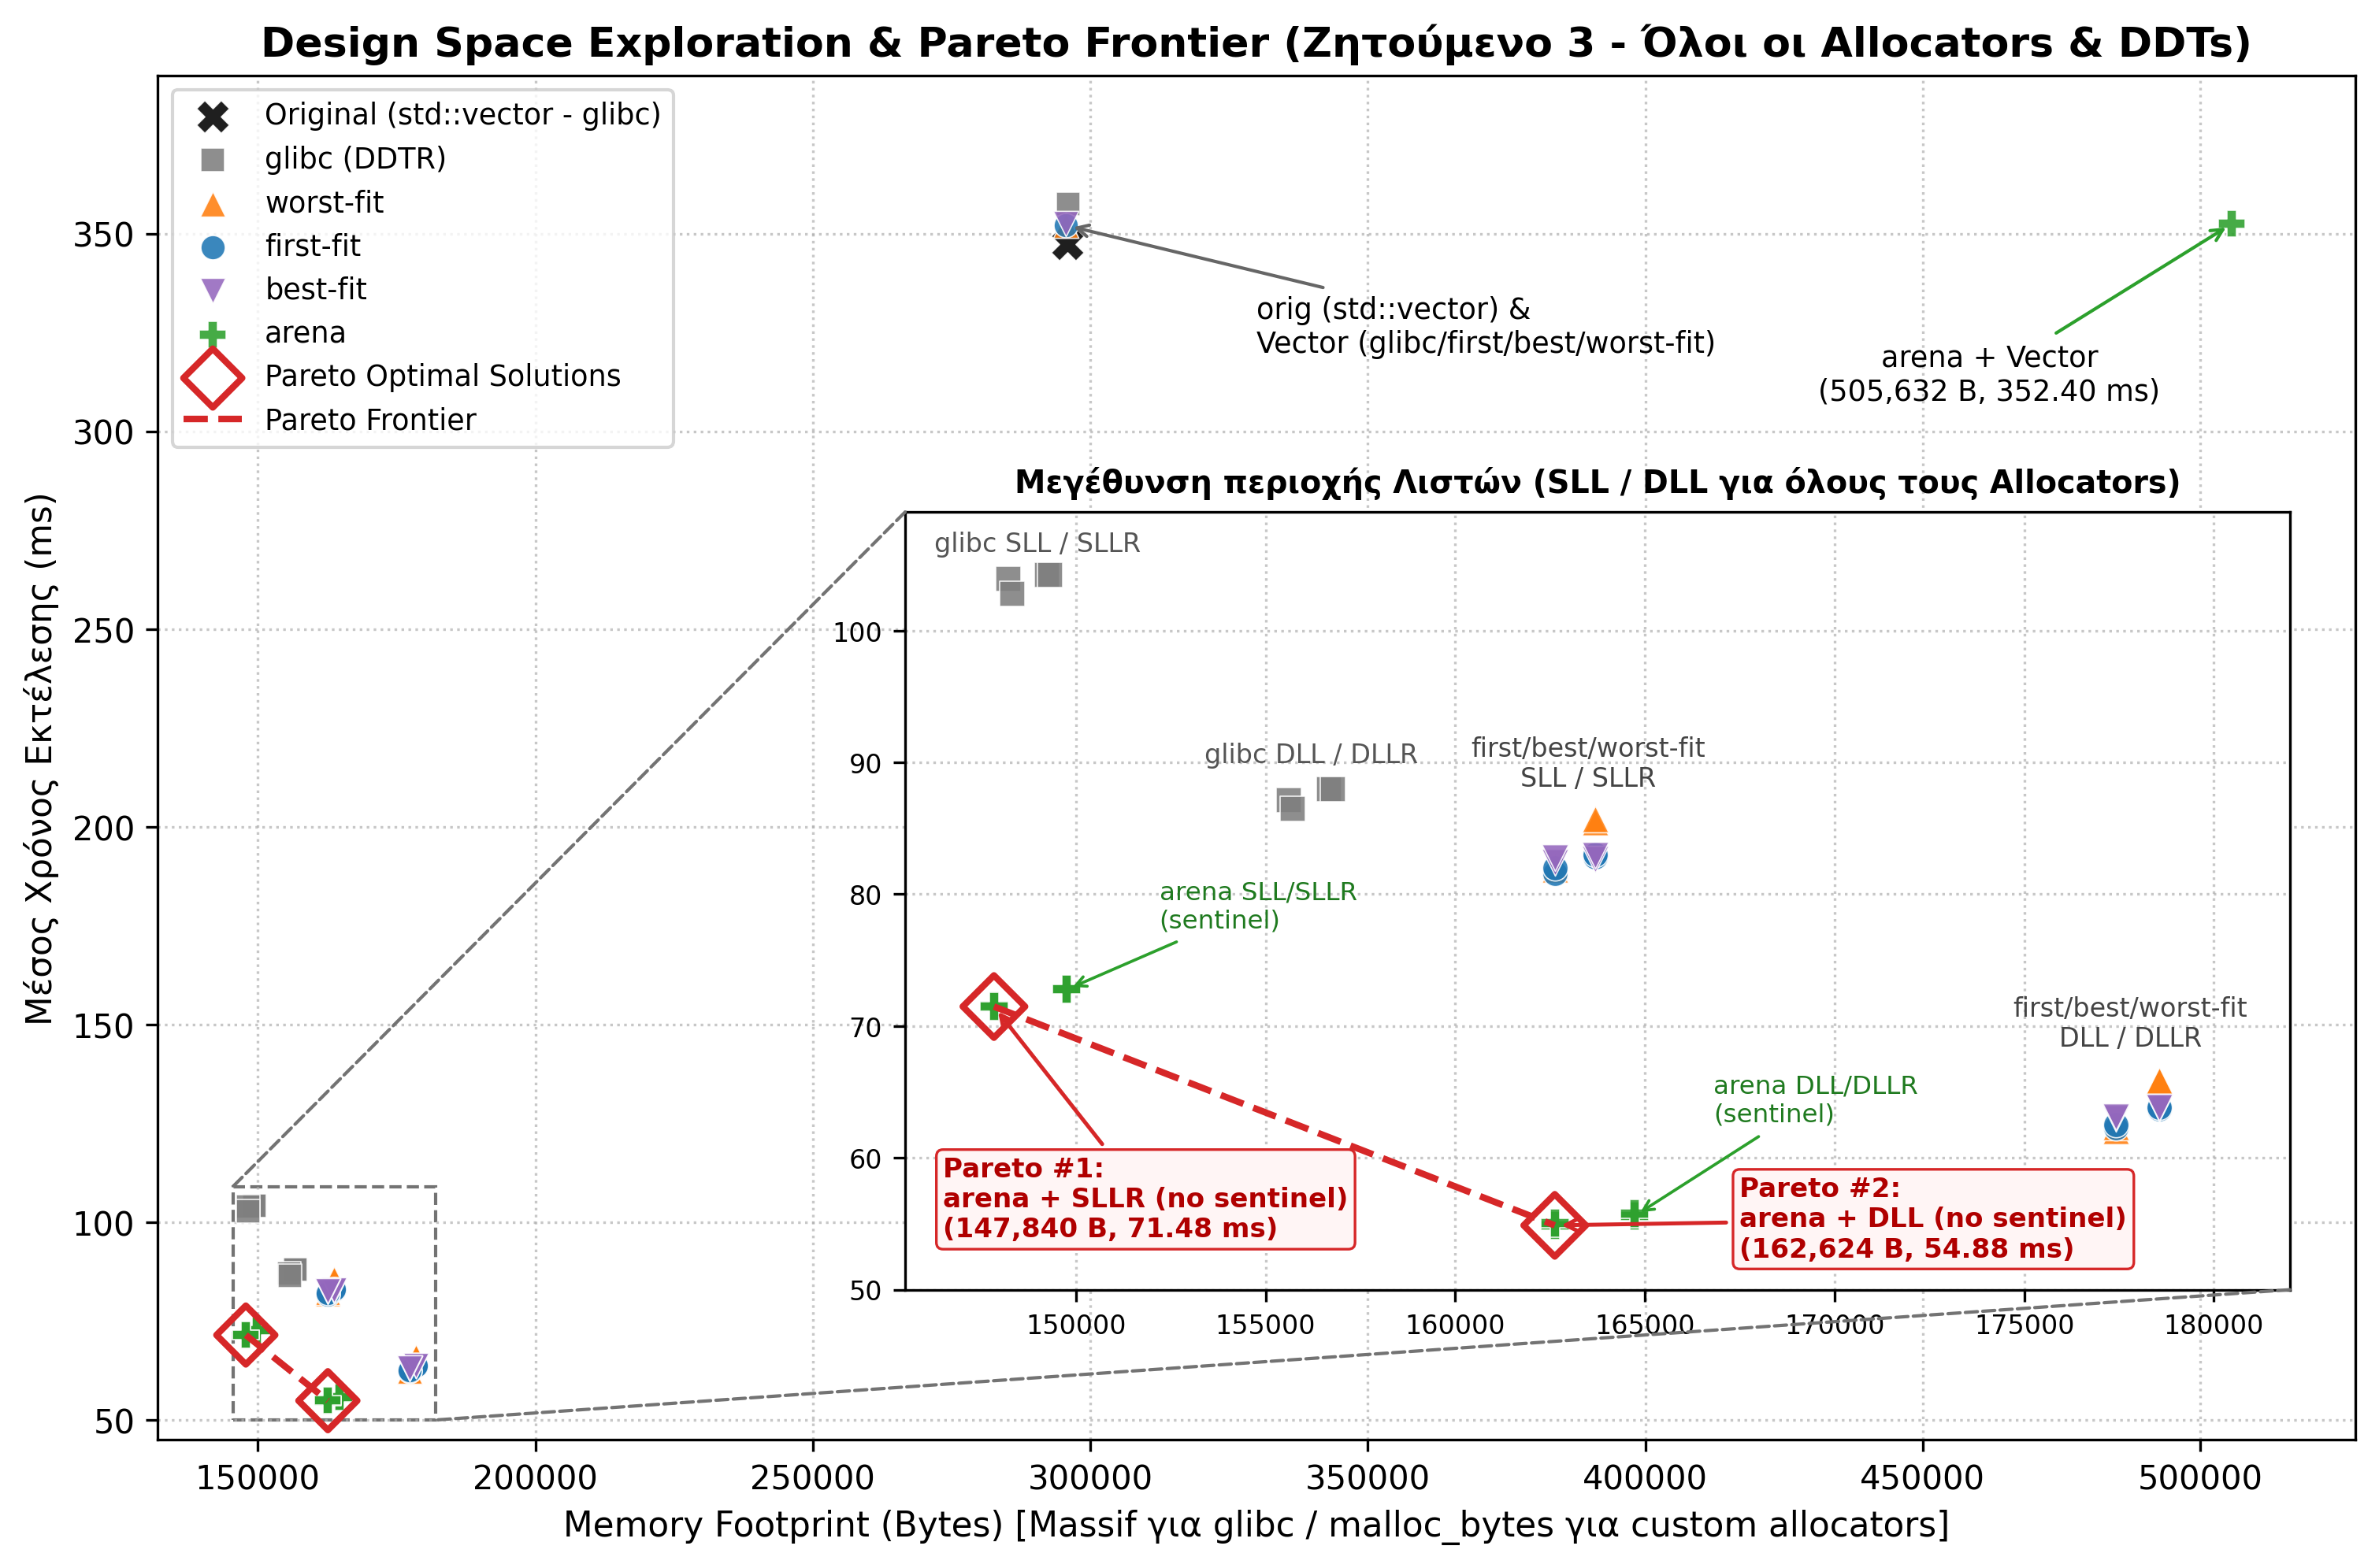
\includegraphics[width=0.8\linewidth]{pareto_q3}
\caption{Pareto Frontier (Ζητούμενο 3 - Όλοι οι Allocators και DDTs)}
\label{fig:q3-pareto}
\end{figure}

Σε σύγκριση με την αρχική υλοποίηση (\texttt{std::vector} και \texttt{glibc}), όπου είχαμε μέσο χρόνο εκτέλεσης \qty{347.39}{\milli\second} και μνήμη \qty{295936}{B}, παρατηρούμε ότι η χρήση custom allocators μαζί με συνδεδεμένες λίστες επιφέρει σημαντική βελτίωση τόσο στον χρόνο εκτέλεσης, όσο και στο memory footprint. Το νέο Pareto Frontier αποτελείται από δύο υλοποιήσεις με \texttt{arena} allocator. Η μία υλοποίηση είναι με DLL χωρίς sentinel κόμβο και έχει χρόνο εκτέλεσης \qty{54.88}{\milli\second} και memory footprint \qty{162624}{B}, πετυχαίνοντας speedup $6.33\times$ και μειώνοντας το memory footprint κατά $45.05\%$, ενώ η δεύτερη Pareto optimal υλοποίηση είναι με \texttt{arena} και SLLR χωρίς sentinel κόμβο και έχει χρόνο εκτέλεσης \qty{71.48}{\milli\second} και memory footprint \qty{147840}{B}, δηλαδή speedup $4.86\times$ και μείωση μνήμης κατά $50.04\%$ σε σχέση με το baseline.

Σημειώνουμε ότι στο Vector οι custom allocators βελτιώνουν ελάχιστα τον χρόνο εκτέλεσης, καθώς και ότι οι καθαρές αστοχίες της LLC παραμένουν σχεδόν σταθερές.

Λαμβάνοντας υπόψη τα παραπάνω, είναι ξεκάθαρο ότι η προτιμότερη επιλογή allocator για την εφαρμογή NMS είναι ο \texttt{arena} σε συνδυασμό με DLL χωρίς sentinel κόμβο αν θέλουμε ελάχιστο χρόνο ή με SLLR χωρίς sentinel κόμβο αν θέλουμε ελάχιστη μνήμη, καθώς αυτές οι δύο υλοποιήσεις κυριαρχούν απολύτως έναντι των υπολοίπων (βλ. Σχήμα \ref{fig:q3-pareto}).

Η ανωτερότητα όλων των custom allocators έναντι της \texttt{glibc} στις συνδεδεμένες λίστες (βελτίωση κατά \qty{18.57}{\milli\second} με \qty{32.39}{\milli\second}) οφείλεται στο ότι η \texttt{glibc} είναι allocator γενικού σκοπού με επιπλέον overhead διαχείρισης. Συγκεκριμένα, ο \texttt{arena} ταιριάζει ιδανικά στην \texttt{nms()}, καθώς εξυπηρετεί κάθε \texttt{malloc()} σε σταθερό χρόνο $O(1)$ χωρίς διάσχιση \texttt{free\_list} και χωρίς 16-byte header ανά κόμβο, εξοικονομώντας \qty{14784}{B} στις λίστες χωρίς sentinel έναντι των free-list allocators. Μεταξύ των \texttt{first-fit}, \texttt{best-fit} και \texttt{worst-fit}, οι χρόνοι είναι παρόμοιοι και το \texttt{malloc\_bytes} πανομοιότυπο, με τον \texttt{first-fit} (μέσος όρος \qty{72.72}{\milli\second} στις λίστες) να προηγείται οριακά του \texttt{best-fit} (\qty{73.07}{\milli\second}, χάρη στη συνθήκη άμεσης διακοπής σε exact fit) και του \texttt{worst-fit} (\qty{73.91}{\milli\second}, που σαρώνει πάντοτε ολόκληρη τη λίστα). Μεταξύ των δύο Pareto optimal λύσεων, η επιλογή \texttt{arena} με DLL χωρίς sentinel (\qty{54.88}{\milli\second}, \qty{162624}{B}) προσφέρει τον καλύτερο σχεδιαστικό συμβιβασμό για εφαρμογή πραγματικού χρόνου, καθώς με μόλις \qty{14784}{B} επιπλέον μνήμης μειώνει τον χρόνο εκτέλεσης κατά \qty{16.60}{\milli\second} σε σχέση με την \texttt{arena} με SLLR χωρίς sentinel.

Καθώς το Massif δεν βλέπει τη μνήμη που γίνεται allocate με την mmap, σε κάθε custom allocator έχουμε υλοποιήσει counters που μετράνε τα Bytes που έγιναν allocate από την mmap (\texttt{mmap\_bytes}) και τα Bytes που χρησιμοποιούν πράγματι οι allocators (\texttt{malloc\_bytes}). Παρατηρούμε ότι καθώς οι allocators δεσμεύουν μνήμη με mmap σε πολλαπλάσια του \qty{1}{MB}, αρκεί μόνο ένα mmap chunk σε κάθε περίπτωση το οποίο μένει εν πολλοίς αναξιοποίητο καθώς οι allocators χρησιμοποιούν πραγματικά πολύ λιγότερη μνήμη. Για παράδειγμα, στο \texttt{arena} με SLLR χωρίς sentinel κόμβο έχουμε \texttt{malloc\_bytes} ίσο με \qty{147840}{B}. Διαπιστώνουμε, λοιπόν, πως θα μπορούσαμε να περιορίσουμε το memory footprint στο λειτουργικό ελαττώνοντας το \texttt{MMAP\_BYTES} σε τιμές πολύ μικρότερες του \qty{1}{MB}.

Όσον αφορά τη διαχείριση των free blocks από κάθε allocator, διακρίνουμε δύο περιπτώσεις. Οι \texttt{first-fit}, \texttt{best-fit} και \texttt{worst-fit} κρατάνε όλα τα ελεύθερα blocks στη συνδεδεμένη λίστα \texttt{free\_list} η οποία είναι ταξινομημένη κατά διεύθυνση μνήμης. Η \texttt{malloc()} ψάχνει στη λίστα ένα ελεύθερο block που χωράει (το πρώτο, το μικρότερο ή το μεγαλύτερο αναλόγως αν έχουμε \texttt{first-fit}, \texttt{best-fit} ή \texttt{worst-fit} αντίστοιχα) και αν αυτό είναι αρκετά μεγαλύτερο, τότε το κάνει split και αφήνει το ελεύθερο κομμάτι στη λίστα. Αν δεν βρει κομμάτι που να χωράει, δεσμεύει ένα νέο chunk μέσω mmap. Η \texttt{free()} βάζει το block πίσω στη λίστα και αν υπάρχει free block δίπλα του, τα ενώνει. Αντιθέτως, στο \texttt{arena} δεν έχουμε \texttt{free\_list}. Η \texttt{malloc()} απλά δεσμεύει μνήμη από το σημείο που δείχνει το offset \texttt{pos} και αυξάνει το offset και τον μετρητή δεσμευμένων blocks \texttt{live}. Η \texttt{free()} δεν αποδεσμεύει τα blocks, απλά μειώνει τον μετρητή \texttt{live} και το chunk επαναχρησιμοποιείται από την αρχή όταν ο μετρητής γίνει ίσος με μηδέν.

\section{Χρήση Flag αντί για erase}
Καθώς η επίδοση και η μνήμη που χρειάζεται η εφαρμογή εξαρτάται από τις προσβάσεις στη μνήμη, κάνουμε μια αλλαγή στο πρόγραμμα ώστε να εξετάσουμε εάν αλλάζει η συμπεριφορά του και κατ' επέκταση το Pareto frontier. Συγκεκριμένα, αλλάζουμε την \texttt{nms()} ώστε να μην κάνει erase τα απορριμμένα candidate boxes, αλλά απλώς να τα σημαδεύει με ένα flag σε ένα vector το οποίο περιέχει ένα unsigned char για κάθε box, με 1 για τα απορριμμένα boxes και 0 για τα υπόλοιπα. Τα συγκεντρωτικά αποτελέσματα παρουσιάζονται στον Πίνακα \ref{tab:q4-results}.

\begin{table}[H]
    \centering
    \scriptsize
    \renewcommand{\arraystretch}{0.88}
    \resizebox{\textwidth}{!}{%
    \csvreader[
        tabular=llcccccccc,
        table head=\toprule Allocator & DDT & Χρόνος (ms) & Var ($\text{ms}^2$) & Mem (B) & mmap (B) & LLC & LLC (\texttt{runs=0}) & Net LLC & Frag. (\%) \\\midrule,
        table foot=\bottomrule,
        late after line=\\
    ]{ddtr_q4_results.csv}{}
    {\csvcoli & \csvcolii & \csvcoliii & \csvcoliv & \csvcolv & \csvcolvi & \csvcolvii & \csvcolviii & \csvcolix & \csvcolx}%
    }
    \caption{Μετρήσεις απόδοσης, μνήμης, προσβάσεων και fragmentation για το Ζητούμενο 4 (\texttt{-DNMS\_FLAG})}
    \label{tab:q4-results}
\end{table}

Από τις μετρήσεις του Πίνακα \ref{tab:q4-results} παρατηρούμε ότι η αντικατάσταση του \texttt{erase()} με τον πίνακα \texttt{Flags} μεταβάλλει ριζικά τη συμπεριφορά των δομών δεδομένων:
\begin{itemize}
\item \textbf{Vector:} Επιτυγχάνεται επιτάχυνση της τάξης του $3.98\times$ με $4.23\times$ (από \qty{352.08}{\milli\second} με \qty{357.40}{\milli\second} σε \qty{83.31}{\milli\second} με \qty{89.87}{\milli\second}), καθώς εξαλείφονται πλήρως οι $O(N)$ μετακινήσεις των 152-byte δομών \texttt{Detection} σε κάθε απόρριψη. Το μέγιστο memory footprint παραμένει αμετάβλητο στη \texttt{glibc} (\qty{295992}{B}) και στους free-list allocators (\qty{295616}{B}), ενώ στον \texttt{arena} αυξάνεται ελαφρώς στα \qty{508896}{B}.
\item \textbf{SLL / SLLR:} Οι απλά συνδεδεμένες λίστες επιταχύνονται κατά \qty{12}{\milli\second} με \qty{16}{\milli\second} σε όλους τους allocators (π.χ. η \texttt{arena} με SLLR χωρίς sentinel κόμβο μειώνεται από \qty{71.48}{\milli\second} σε \qty{59.42}{\milli\second}), επειδή αποφεύγουν τη δαπανηρή διαγραφή στοιχείου της SLL.
\item \textbf{DLL / DLLR:} Αντιθέτως, οι διπλά συνδεδεμένες λίστες επιβραδύνονται κατά \qty{6}{\milli\second} με \qty{8}{\milli\second} (π.χ. η \texttt{arena} με DLL χωρίς sentinel αυξάνεται από \qty{54.88}{\milli\second} σε \qty{62.86}{\milli\second}). Αυτό οφείλεται στο γεγονός ότι χάνουν το πλεονέκτημα της $O(1)$ διαγραφής που συρρίκνωνε τη λίστα σε κάθε βήμα, με αποτέλεσμα ο εμφωλευμένος βρόχος να διασχίζει πλέον όλους τους απορριμμένους κόμβους ελέγχοντας το \texttt{Flags} vector, διατηρώντας ταυτόχρονα το επιπλέον κόστος των μεγαλύτερων κόμβων.
\item \textbf{Allocators, Μνήμη, Fragmentation και LLC Misses:} Οι παραλλαγές χωρίς sentinel κόμβο παραμένουν ανώτερες σε όλους τους συνδυασμούς, ενώ ο \texttt{arena} διατηρεί την πρωτιά σε ταχύτητα (\qty{59.42}{\milli\second} με \qty{64.32}{\milli\second} στις λίστες), ακολουθούμενος από τους \texttt{first-fit}, \texttt{best-fit}, \texttt{worst-fit} (\qty{68.93}{\milli\second} με \qty{74.71}{\milli\second}) και τη \texttt{glibc} (\qty{87.64}{\milli\second} με \qty{94.20}{\milli\second}). Ο πίνακας \texttt{Flags} προσθέτει μικρή επιβάρυνση στη μνήμη των λιστών (\qty{1536}{B} στη \texttt{glibc}, \qty{1568}{B} στους free-list allocators και \qty{3040}{B} στον \texttt{arena}, καθώς ο τελευταίος δεν επαναχρησιμοποιεί τα ενδιάμεσα buffers του \texttt{Flags} vector). Επειδή το \texttt{mmap\_bytes} παραμένει \qty{1}{MB} (\qty{1048576}{B}), το ποσοστό ανεκμετάλλευτης μνήμης (fragmentation) κυμαίνεται στο $82.82\%$ με $85.61\%$ για τις λίστες ($71.81\%$ για τους free-list allocators και $51.47\%$ για τον \texttt{arena} στο Vector). Τέλος, οι καθαρές αστοχίες της LLC ($\Delta$) παραμένουν πρακτικά σταθερές γύρω στις $185{,}000$ με $193{,}000$.
\end{itemize}

Στο Σχήμα \ref{fig:q4-pareto} απεικονίζονται συγκριτικά τα σημεία της νέας εκδοχής (τρίγωνα) μαζί με τα σημεία του Ζητουμένου 3 (κύκλοι) και τη συνολική καμπύλη Pareto.

\begin{figure}[H]
\centering
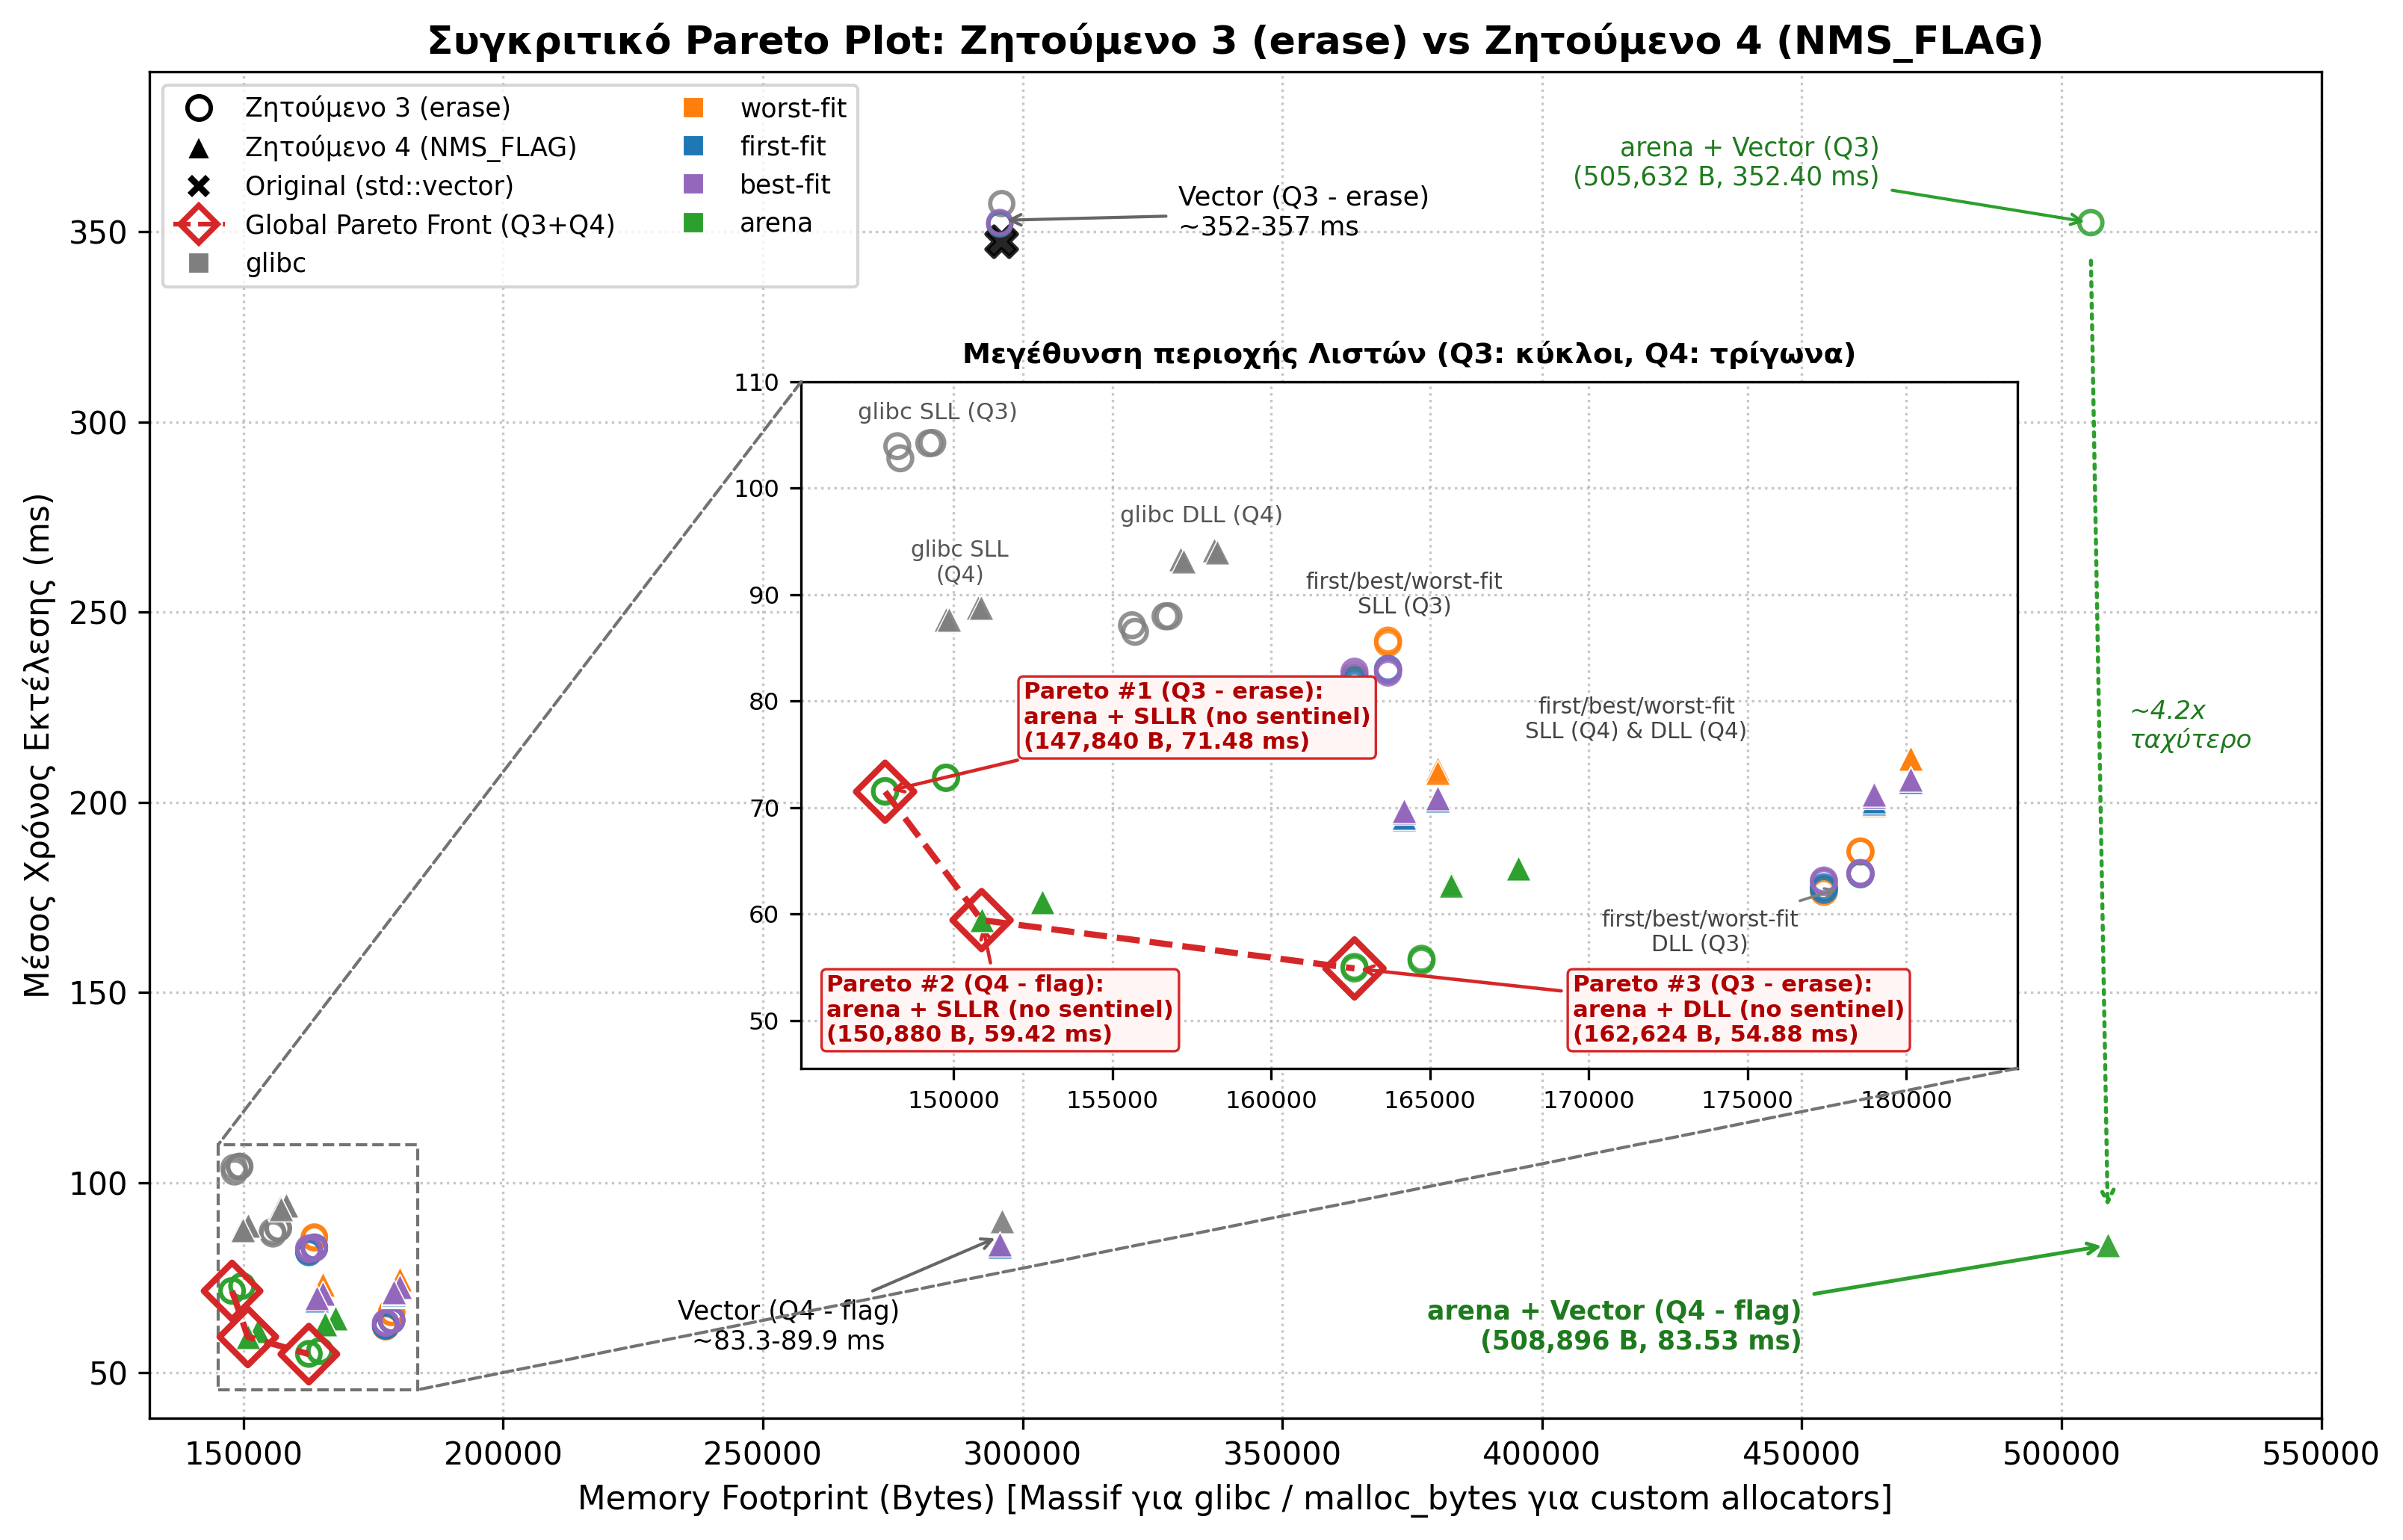
\includegraphics[width=0.9\linewidth]{pareto_q4}
\caption{Συγκριτικό Pareto Frontier μεταξύ Ζητουμένου 3 (\texttt{erase}) και Ζητουμένου 4 (\texttt{NMS\_FLAG})}
\label{fig:q4-pareto}
\end{figure}

Εντός της νέας εκδοχής (\texttt{NMS\_FLAG}), βέλτιστος allocator παραμένει ο \texttt{arena}, ωστόσο η επιλογή της βέλτιστης δομής δεδομένων αλλάζει σε σχέση με τα Ζητούμενα 2 και 3: πλέον οι απλά συνδεδεμένες λίστες χωρίς sentinel κόμβο (\texttt{arena} με SLLR χωρίς sentinel στα \qty{59.42}{\milli\second} και \qty{150880}{B}, με σχεδόν ταυτόσημη επίδοση για την SLL χωρίς sentinel στα \qty{59.50}{\milli\second}) υπερτερούν των διπλά συνδεδεμένων λιστών (\qty{62.71}{\milli\second} με \qty{62.86}{\milli\second} και \qty{165664}{B}) τόσο σε χρόνο όσο και σε μνήμη. Η μεταβολή αυτή εξηγείται από το γεγονός ότι στα Ζητούμενα 2 και 3 η υπεροχή της DLL οφειλόταν αποκλειστικά στον δείκτη \texttt{prev} που επέτρεπε διαγραφή σε χρόνο $O(1)$. Με την κατάργηση του \texttt{erase()}, ο δείκτης \texttt{prev} παύει να προσφέρει όφελος και παραμένει μόνο η επιβάρυνση των μεγαλύτερων κόμβων (επιπλέον \qty{16}{B} ανά κόμβο λόγω ευθυγράμμισης) και των περισσότερων εγγραφών κατά την κατασκευή και την ταξινόμηση της λίστας.

Εξετάζοντας συνολικά και τις δύο εκδοχές (Σχήμα \ref{fig:q4-pareto}), το κοινό Pareto Frontier αποτελείται από τρία σημεία, όλα με χρήση του \texttt{arena} allocator:
\begin{enumerate}
\item \texttt{arena} + SLLR χωρίς sentinel με \texttt{erase} (\qty{147840}{B}, \qty{71.48}{\milli\second}), που ελαχιστοποιεί τη μνήμη.
\item \texttt{arena} + SLLR χωρίς sentinel με \texttt{NMS\_FLAG} (\qty{150880}{B}, \qty{59.42}{\milli\second}), που αποτελεί την ενδιάμεση βέλτιστη λύση μειώνοντας τον χρόνο της SLLR κατά \qty{12.06}{\milli\second} με μόλις \qty{3040}{B} επιπλέον μνήμης.
\item \texttt{arena} + DLL χωρίς sentinel με \texttt{erase} (\qty{162624}{B}, \qty{54.88}{\milli\second}), η οποία παραμένει η ταχύτερη υλοποίηση ολόκληρης της άσκησης (speedup $6.33\times$ έναντι του baseline), καθώς η φυσική αφαίρεση των απορριμμένων boxes μειώνει δραστικά τις επαναλήψεις του εμφωλευμένου βρόχου χωρίς το κόστος διάσχισης ήδη απορριμμένων στοιχείων.
\end{enumerate}

\end{document}
